\section{Introduction}
\label{sec:Introduction}

%%%%%%%%%%%%%%%%%%%%%%%%%%%%%%%%%%%%%%%%%%%%%%%%%%%%%%%%%%%%%%%%%%%%%%%%%%%%%%%%
%% \rkc{Part 1.1: Motivation and SAL/CAL/FPF. Editing TBD.}

Conventionally, the design of data structures and algorithms is chiefly focused on performance, which is of significantly diminished concern in proof assistants.
%
As such, proof assistants often use entirely different data structures than those of conventional settings, with a focus on simplicity or useful proof-theoretic properties.

Consider dictionaries, which---among a broad range of purposes---are often used for implementing type contexts and evaluation environments.
%
The most basic representation for a dictionary, an \emph{\sal}, comprises a list of key-value pairs~\citep{XXX,XXX,XXX}.
%
Association lists are simple to create, manipulate, and reason about.
%
But because they allow duplicate bindings for the same key and they are sensitive to the order of insertions, many distinct \sal{}s represent the same semantic mapping.
%
For example, the association lists on the first two lines of \autoref{fig:intro-example}%
%
%% ---and illustrated below in \autoref{fig:uneq}---
%
are two ways (among many others) to represent a dictionary with three particular bindings.

%% %% \begin{figure}[b]
\begin{figure}[h]
  \centering
  \begin{tikzpicture}[nodes = {align = left}]
    %% \node [scale=.45]
    \node [scale=.33]
    {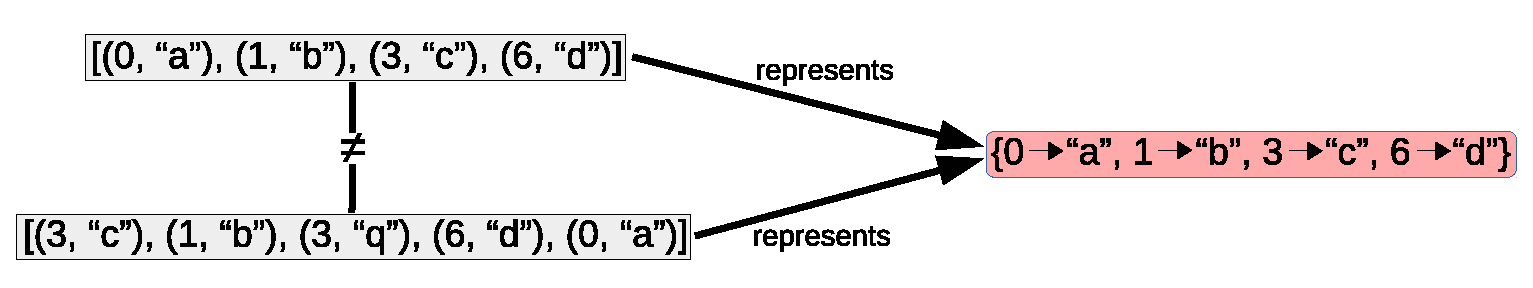
\includegraphics{figs/unequal.eps}};
  \end{tikzpicture}
  \caption{Two distinct \sal{}s representing the same semantic mapping. \rkc{Let's show the first two rows from Fig 1. And let's fit this into one column.}}
  \label{fig:uneq}
\end{figure}


\newcommand{\no}
  %% {No}
  %% {}
  {\color{lightgray}\phantom{$^*$}\xmark\phantom{$^*$}}
\newcommand{\noIO}
  %% {\color{lightgray}\phantom{$^*$}\xmark$^*$}
  {{\color{lightgray}\phantom{$^*$}\xmark}\footnotemark[3]} % 3 is hard-coded, but I see no other way
\newcommand{\yes}
  %% {Yes}
  %% {\phantom{*}\cmark\phantom{*}}
  {\phantom{$^-$}\cmark\phantom{$^-$}}
\newcommand{\yesMinus}
  %% {Yes*}
  %% {\phantom{*}\cmark*}
  {\phantom{$^-$}\cmark$^-$}
\newcommand{\yesPlus}
  %% {Yes*}
  %% {\phantom{*}\cmark*}
  {\phantom{$^-$}\cmark$^+$}
\newcommand{\eq}
  %% {Decidable equality}
  %% {Eq K}
  %% {(=) : (K,K) -> Bool}
  {$(=)$}
\newcommand{\ord}
  %% {Orderable}
  %% {Eq K, Ord K}
  %% {(=),(<) : (K,K) -> Bool}
  {$(=), (<)$}
\newcommand{\isoNat}
  %% {Bijects to naturals}
  %% {K $\leftrightarrow$ Nat}
  {$f\hspace{0.02in}\!:\!\hspace{0.02in}K \leftrightarrow \textit{Nat}$}

\newcommand{\header}[1]
  {\makebox[0.67in]{#1}}
\newcommand{\headers}[6]
  {&\header{#1}&\header{#2}&\header{#3}&\header{#4}&\header{#5}&\header{#6}}

%% \begin{figure}[H]
\begin{figure*}[t]
  \begin{tabular}{ l || c | c | c | c | c || c}
  \multirow{2}{*}{}
           & \multicolumn{5}{c||}{\footnotesize Client Usage}
           & {\footnotesize Implementation} \\ \cline{2-7}
   \headers{\total}{\extensional}{\decidable}{\destructible}{Key Type $K$}{Simple}    \\ \hline
   \Sal    & \yes   & \no        & \yes      & \yes         & \eq       & \yesPlus  \\ %% \hline
   \Cal    & \no    & \yes       & \yes      & \yes         & \ord      & \yesMinus \\ %% \hline
   \Fpf    & \noIO  & \yes       & \no       & \no          & \eq       & \yes      \\ \hline
   %% \Fpfk   & \no    & \yes       & \yes      & \yes         & \ord      & \simple     \\ \hline
   \Dd     & \yes   & \yes       & \yes      & \yesMinus    & \isoNat   & \no
  \end{tabular}
  \caption{Properties of dictionary representations.}
  \label{fig:prop-summary}
\end{figure*}
%% \end{figure}
 %% here to force layout on p.2

To establish a one-to-one correspondence between association lists and semantic mappings, one solution~\citet{XXX,XXX,XXX} is to maintain a \emph{canonical} form that is semantically valid and unique, namely, a list in which there are no duplicate keys and, furthermore, where keys are in sorted order.
%
The second association list described in \autoref{fig:intro-example} is one such example.
%
This approach allows proofs with canonical association lists to use built-in equality for semantic equivalence, at the expense of extending the underlying list type---which allows arbitrary, possibly invalid lists---with a proof of validity that refines the coarser type.

A third conventional solution is to represent dictionaries as finite partial functions~\citep{XXX,XXX,XXX}.
%
The third line of \autoref{fig:intro-example} depicts a nested lambda-expression that serves as the ``lookup table.'' 
%
Assuming the additional postulate of \emph{functional extensionality}~\cite{XXX}, this representation allows for the use of built-in equality for semantic equivalence.\footnote{\hspace{0.01in}%
%
This postulate is consistent with the constructive calculi underlying most popular proof assistants~\citep{XXX}.
%
}
%
However, a plain function type does not rule out the possibility of the term being a \emph{non-}finite map, possibly requiring additional proofs of validity as with canonical association lists.\footnote{\hspace{0.01in}%
%
This often isn't a problem in practice -- in cases where the dictionary is not iterated or otherwise destructed, an infinite dictionary will generally work just as well as a finite one,
%
so it's not actually necessary to retain a proof that the dictionary is finite.
%
}
%
Worse is the fact that, unlike either association list representation, equality of partial functions is not decidable.
%
The function type could be refined with its domain---\ie{}~a canonical list of keys---but would then suffer the drawbacks of manipulating validity proofs \`{a} la canonical association lists while being needlessly complicated.

In some cases, the aforementioned drawbacks are minor or can be worked around.
%
But developing large proofs is challenging, so any stumbling block---the inability to use built-in equality to establish semantic equivalence of two objects, or the awkwardness of packaging proof terms with data (noting the difficulties that arise from proof relevance)---can cause exorbitant increases in verbosity, time, effort, and accidental complexity.

%% Because the representations of semantically equivalent dictionaries are not necessarily equal, proofs involving association lists may not use a built-in equality to distinguish them.
%% 
%% - are typically implemented in one of the following manners: (TODO source for each)

%% The \sal~ (\SAL) solution is perhaps the most common, being trivially simple. Furthermore:
%% %\begin{itemize}
%%  (1) any \SAL~ that type-checks represents a valid mapping,
%%        so there's no need to refine the dict with a proof term that asserts its validity,
%%  (2) it's trivial to destruct and iterate,
%%  (3) checking semantic equivalence of two dicts, while non-trivial, is decidable and not too difficult.
%% %\end{itemize}

%% Since performance is often not a concern,
%% we have an opportunity to reassess the core criteria by which data structures are judged. Chiefly, these
%% new criteria will focus on alleviating or eliminating difficulties that crop up in the development of
%% proofs. In the \nameref{sec:Problem} section, we discuss several of these properties and argue for their
%% conceptual and practical importance.

%% The \cal~ (\CAL) and \fpf~ (\FPF) solutions (as well as ours) are set-like - i.e. they are insensitive
%% to duplication and ordering of insertions. As such, semantically equivalent dicts are also equal according
%% to the built-in equality primitive\footnote{Finite partial functions require the additional postulate of
%% \emph{functional extensionality}, which can be postulated
%% at essentially no cost given that it's been proven consistent with the constructive calculi underlying most
%% popular proof assistants (TODO SOURCE)}. However, \CAL~ and \FPF~ have other drawbacks.
%% If used as data, a \CAL~ must be refined with a proof of validity to ensure that it is ordered and deduped,
%% while equality is not decidable for {\FPF}s. In the \nameref{sec:Problem} section we discuss the difficulties
%% that arise from these drawbacks.


%%%%%%%%%%%%%%%%%%%%%%%%%%%%%%%%%%%%%%%%%%%%%%%%%%%%%%%%%%%%%%%%%%%%%%%%%%%%%%%%
%% \rkc{Part 1.2: Summary of Design Goals. Editing TBD.}

Ideally, when working in a proof assistant, an implementation of a data structure---dictionaries in particular for this paper---would satisfy the following properties:

\newcommand{\designGoal}[1]
  {\textbf{\emph{#1:}}}

\begin{enumerate}

\item
%
\designGoal{\SemTot}
%
Every term in the representation type is semantically valid, \ie{}~the mapping from terms to their semantic meanings is total.

\item
%
\designGoal{\SemInj}
%
Built-in equality corresponds to semantic equivalence, \ie{} two unequal terms have different semantic meanings.

\item
%
\designGoal{\EqDec}
%
Built-in equality is decidable for the type.

\end{enumerate}

Furthermore, in addition to properties about the external interface of the data structure, it is often useful to retain the ability to inspect, iterate, and manipulate sub-dictionaries.
%
Thus, our final design goal:

\begin{enumerate}

\item[4.]
%
\designGoal{\EzDstr}
%
The ability to decompose a data structure into atomic parts, to facilitate inspection or unrestricted non-additive manipulation, in a sufficiently convenient manner.

\end{enumerate}

\autoref{fig:prop-summary} summarizes the preceding discussion along these dimensions; note that all conventional representations except partial functions can be easily destructed.
%
%% None of the conventional representations satisfies both \SemTot{} and \SemInj{}, let alone the additional properties.
%
%% None of the conventional representations satisfies more than three of the four properties.
%
None of the conventional representations satisfies both \SemTot{} and \SemInj{}, nor more than three of the four properties.


%%%%%%%%%%%%%%%%%%%%%%%%%%%%%%%%%%%%%%%%%%%%%%%%%%%%%%%%%%%%%%%%%%%%%%%%%%%%%%%%
%% \rkc{Part 1.3: Delta Dicts. Editing TBD.}

\parahead{A New Representation}
%
We offer a solution, dubbed \emph{\dds{}}, which achieves the first three of the desired properties, and partially achieves the fourth. 
%
%% A \dd{} is similar to a canonical association list, but instead of storing each literal key value, it stores the \emph{difference} from the previous key, minus 1.
%
A \dd{} can be described as a ``canonical-by-construction'' association list: instead of storing each literal key value, it stores the \emph{difference} from the previous key, minus 1.
%
For example, compare the canonical association list and \dd{} for the \autoref{fig:intro-example} example:

\vsepRule

%% keep this in sync with Figure 1
\begin{tabular}{ l l }
 \Cal{} & [(1, "a"), (3, "b"), (6, "c")] \\
 \Dd{}  & [(1, "a"), (1, "b"), (2, "c")]
\end{tabular}

\vsepRule

Every well-typed list-of-pairs is a valid \dd{} (\SemTot), thus no proof term is needed to establish validity.
%
Every unique \dd{} represents a unique semantic mapping, thus built-in equality may be used for semantic equivalence (\SemInj).
%
%% there is a bijection between \dd{} terms and finite maps,
%
Furthermore, we can (and do) define a function which determines whether or not two \dds{} are equal (\EqDec).

As summarized in \autoref{fig:prop-summary}, delta dictionaries strike a new balance in this design space.
%
Compared to \cal{}s, \dds{} enjoy \SemTot{}---the lone property among those we identify which \cal{} does not.
%
However, destruction and iteration for \dds{} is substantially more difficult.
%
Furthermore, unlike all of the conventional representations, \dds{} require a bijection to the naturals, not merely an ordering, for their key types.
%
%% Our definition and implementation uses natural numbers for keys, and we illustrate how to use bijections to the naturals as a way of supporting strings, integers, or other key types that can be bijected to the naturals without great difficulty.
%
Lastly, though not a concern from a client's perspective, the implementation of delta dictionaries is considerably more involved than the conventional approaches.

%% than it is with the {\SAL}s or {\CAL}s, for which these operations are trivial ({\FPF}s cannot be properly destructed at all).

%% Naturally, \dds~ have some drawbacks as well.

%% Although most types that are suitable for use as keys in the first place can be bijected to the
%% naturals, for some types defining this bijection may be too awkward or cumbersome, in which case \dds~ may
%% be a poor choice.

%% As with the drawbacks of the other solutions, this one is
%% discussed further in the \nameref{sec:Problem} section.

\parahead{Outline}
%
%% Next, we describe the core operations for delta dictionaries in \autoref{sec:DD} and the relevant metatheory in \autoref{sec:DD:props}.
%
Next, we describe the core operations for delta dictionaries and the relevant metatheory in \autoref{sec:DD}.
%
In \autoref{sec:CaseStudy}, we describe a small case study in proof development that motivated the design of delta dictionaries.
%
Finally, we conclude in \autoref{sec:Discussion} with a discussion of related work.
%
%% Our implementation and proofs are formalized in Agda and available in the anonymous supplementary materials.


%% {\color{gray}
%% 
%% \subsection{\rkc{Grab Bag of Text}}
%% 
%% %% \section{Problem}
%% %% \subsection{Problem}
%% %% \label{sec:Problem}
%% 
%% \rkc{1}
%% 
%% Data structures can possess or lack a wide range of properties that make them easier or harder to work with
%% when proving metatheory. Naturally, when possible, data structures should be chosen that posess those
%% properties which make the task at hand easier. Achieving this requires identifying the valuable properties,
%% what it is that makes them valuable, and finding or inventing data structures which possess those properties.
%% We hold that this is a broad topic of
%% research, which we illustrate in the particular context of choosing an implementation for a dictionary. In
%% this context, we identify, according to both conceptual and practical considerations, four important and
%% discriminating properties that a dictionary implementation may or may not possess:
%% TODO there's a good chance some of these properties have been named somewhere else. We should make sure we
%% don't try and coin terms for anything that's already been defined somewhere.
%% 
%% % TODO we may decide that the conceptual and practical benefits of decidable equality are so obvious or
%% % self-evident that we don't need any further discussion of that property
%% 
%% %% \subsection{Conceptual Importance}
%% %% \label{sec:Problem:concept}
%% 
%% \rkc{2}
%% 
%% In \autoref{sec:Problem:pract}, we illustrate practical problems and benefits under the particular context
%% of choosing an implementation for dictionaries. But first, it's worth exploring conceptual aspects that
%% apply to the general case. These conceptual aspects capture the spirit of practical considerations and
%% motivate the search for solutions that are not merely serviceable but elegant, moral, and insightful.
%% 
%% \subsubsection{\SemTot}
%% \label{sec:Problem:concept:SemTot}
%% TODO something something "making impossible states impossible", i think allusion to the right parts out of that
%% video will suffice to make the point here
%% 
%% \subsubsection{\SemInj}
%% \label{sec:Problem:concept:SemInj}
%% TODO something something it yields arbitrariness, which is not always wrong but which is unaesthetic and, when
%% avoidable, undesirable. It also allows for a semantic meaning to be represented by a concrete thing that is
%% needlessly verbose and complicated.
%% 
%% \subsubsection{\EqDec}
%% \label{sec:Problem:concept:EqDec}
%% The languages of proof assistants generally pride themselves on being total and constructive, on emphasizing
%% the knowable and demonstrable over the mysterious and hypothetical.
%% 
%% \subsubsection{\EzDstr}
%% \label{sec:Problem:concept:EzDstr}
%% TODO We need to clearly explain what we're talking about here, and clarify stuff like "facilitate inspection"
%% and "unrestricted non-additive manipulation". Aside from these clarifications, we won't say much else - in
%% this case the conceptual value largely boils down to the practical value.
%% 
%% %Finally, because they guarantee the \emph{structural properties} \emph{contraction} and
%% %\emph{exchange}, \dds~ are inherently inappropriate for substructural logics/judgments that reject one or
%% %both of those properties. In these cases, the naive solution's sensitivity to duplication and/or ordering is
%% %a feature, not a bug, and that solution becomes not only the natural solution but the morally correct one.
%% %Future work could explore the possibility of data structures that uphold one of these properties but not the
%% %other.
%% 
%% }
